\appendix
%\begin{landscape}
\chapter{Testergebnisse}
\section{\ac{snr}}
%\lstinputlisting[caption=Matlab \ac{snr} Test Skript, escapechar=, label=lst:matlab_snr, style=Matlab]{sourcecode/Test_SNR.m}
\begin{figure}[ht!]
	\centering
	\begin{subfigure}[t!]{0.82\textwidth}
		\centering
  		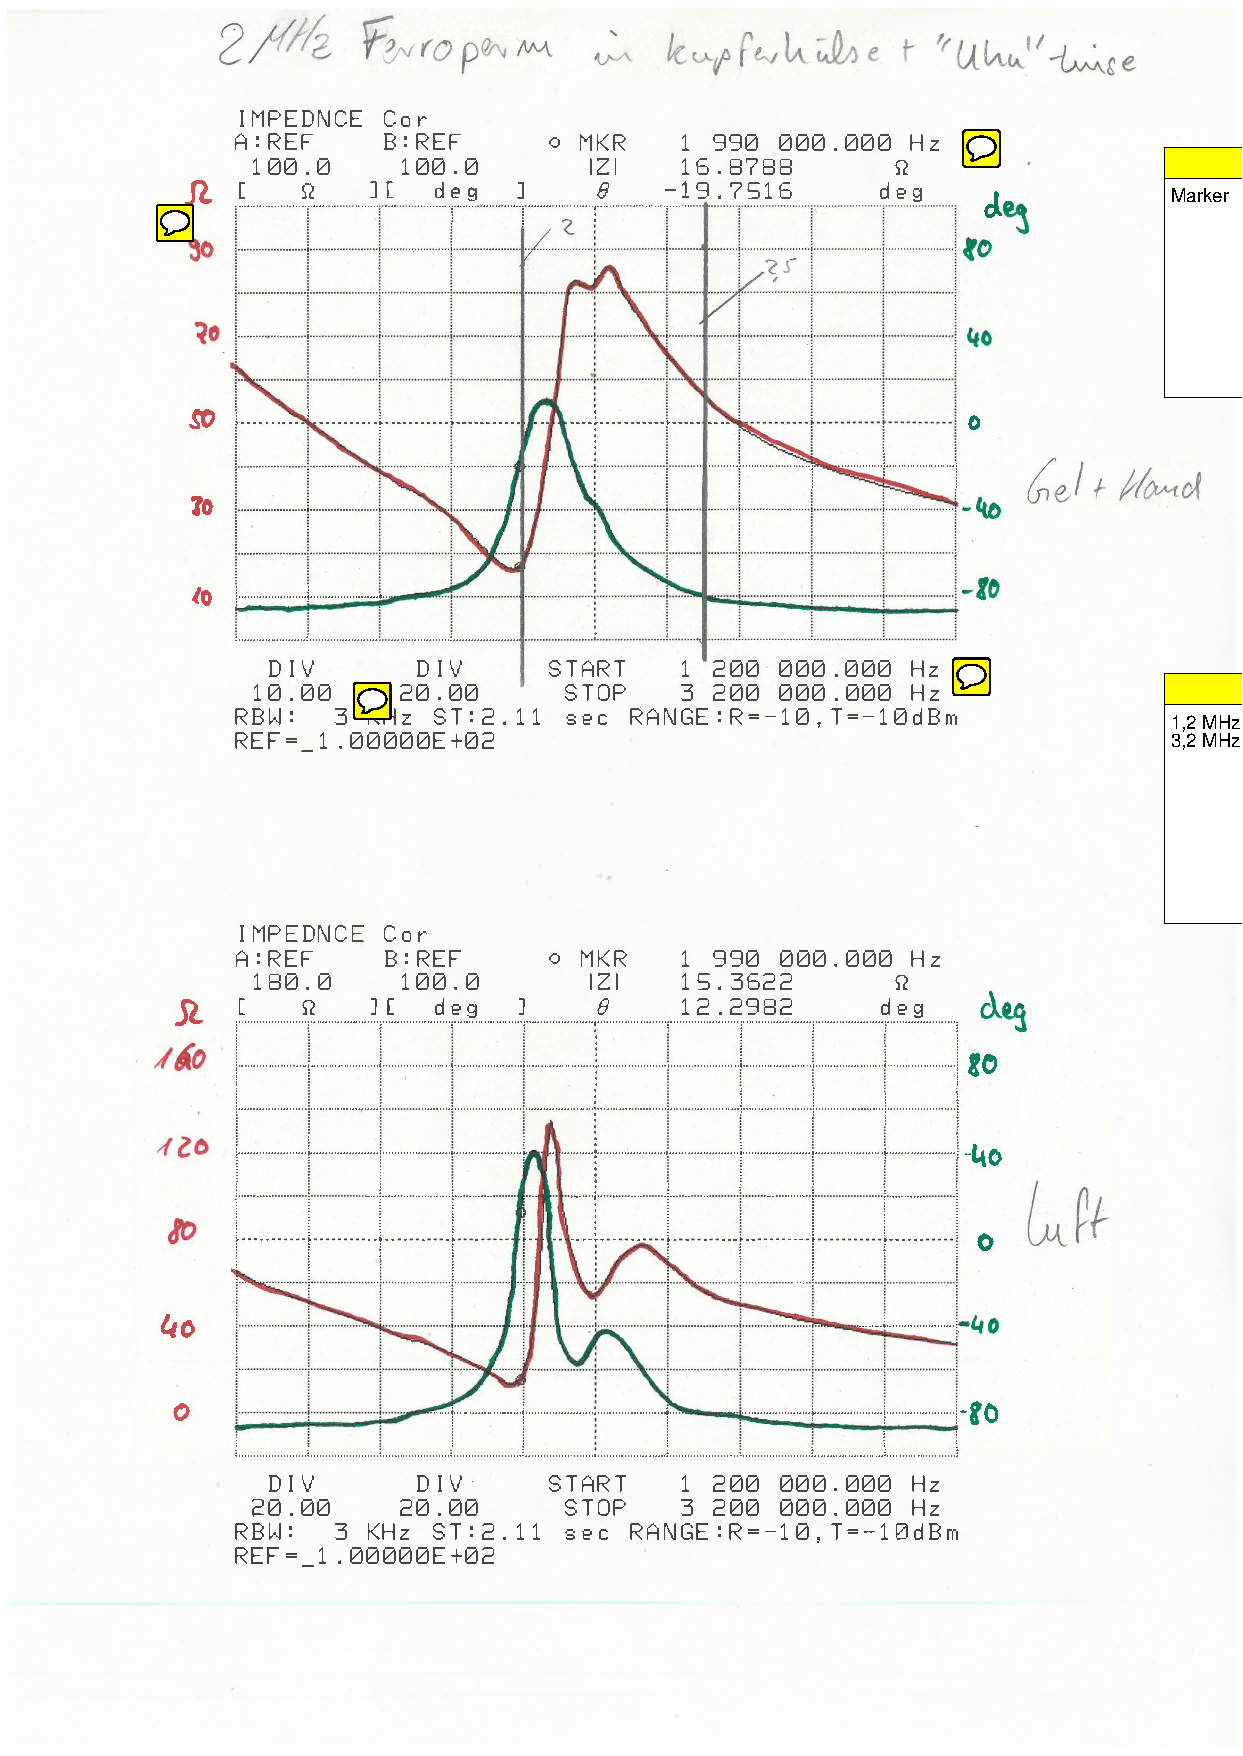
\includegraphics[page=1,width=\textwidth, trim= 31mm 178mm 36mm 22mm, clip=true]{attachment/Impedanzen_Sonden.pdf}% \\[.5cm]
 		\caption{Gel + Hand}
 		\label{fig:2_sig}
  	\end{subfigure}
  	\begin{subfigure}[t!]{0.82\textwidth}
	  	\centering
  		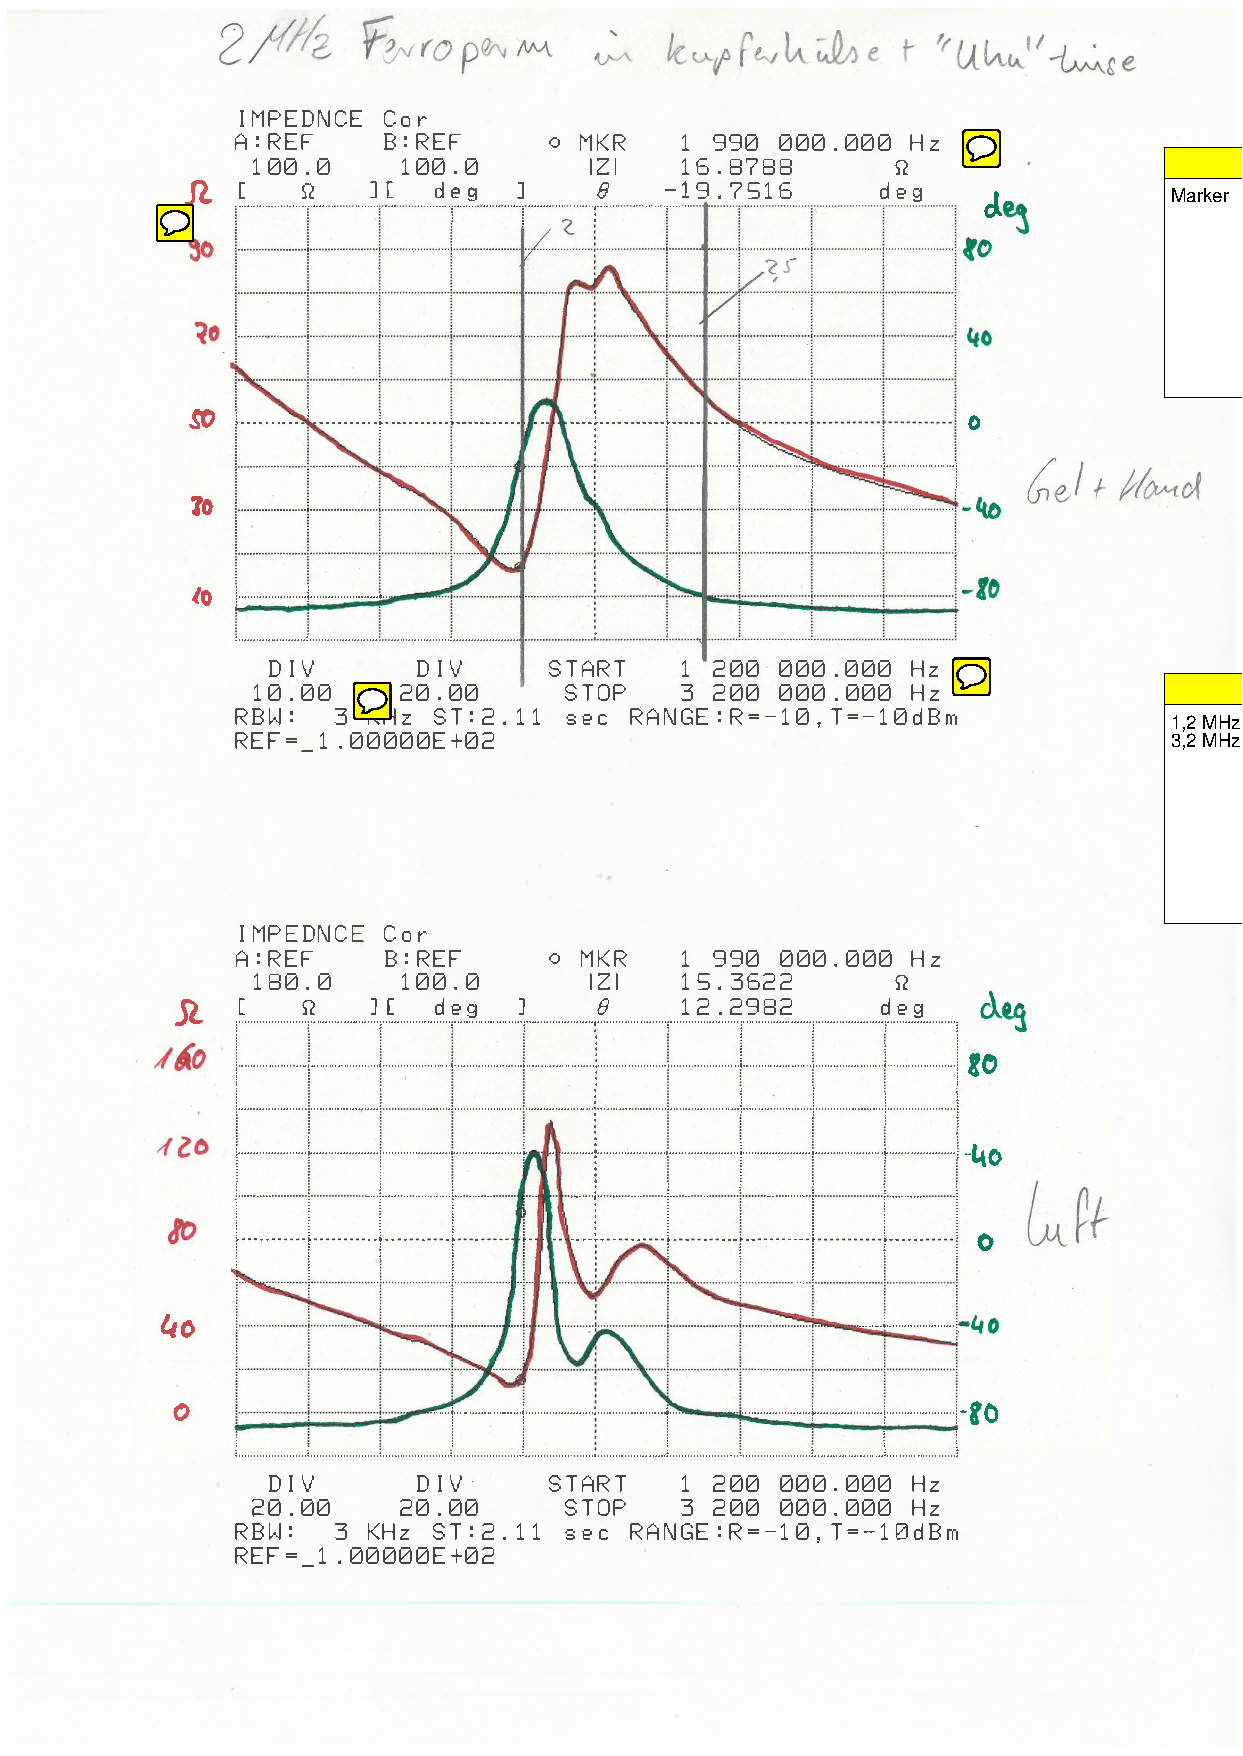
\includegraphics[page=1,width=\textwidth, trim= 26mm 40mm 36mm 160mm, clip=true]{attachment/Impedanzen_Sonden.pdf} %\\[.5cm]
  		\caption{Luft}
 		\label{fig:snr_2_script}
  	\end{subfigure}
  	\caption{2 \ac{mhz} Feroperm Kupferhülse + Uhu-tinse (page 1)}
\end{figure}
\clearpage

\begin{figure}[ht!]
	\centering
	\begin{subfigure}[t!]{0.82\textwidth}
	  	\centering
  		\includegraphics[page=3,width=\textwidth, trim= 27mm 63mm 37mm 137mm, clip=true]{attachment/Impedanzen_Sonden.pdf} %\\[.5cm]
  		\caption{normal page 3}
 		\label{fig:snr_2_script}
  	\end{subfigure}
  	\begin{subfigure}[t!]{0.82\textwidth}
	  	\centering
  		\includegraphics[page=5,width=\textwidth, trim= 26mm 64mm 37mm 137mm, clip=true]{attachment/Impedanzen_Sonden.pdf} %\\[.5cm]
  		\caption{im Kupferring page 5}
 		\label{fig:snr_2_script}
  	\end{subfigure}
  	\caption{2 \ac{mhz} Kristall (Luft) }
\end{figure}
\clearpage

\begin{figure}[ht!]
	\centering
	\begin{subfigure}[t!]{0.82\textwidth}
	  	\centering
  		\includegraphics[page=6,width=\textwidth, trim= 28mm 178mm 39mm 22mm, clip=true]{attachment/Impedanzen_Sonden.pdf} %\\[.5cm]
  		\caption{Gel + Hand}
 		\label{fig:snr_2_script}
  	\end{subfigure}
  	\begin{subfigure}[t!]{0.82\textwidth}
	  	\centering
  		\includegraphics[page=6,width=\textwidth, trim= 32mm 42mm 39mm 158mm, clip=true]{attachment/Impedanzen_Sonden.pdf} %\\[.5cm]
  		\caption{in Luft}
 		\label{fig:snr_2_script}
  	\end{subfigure}
  	\caption{2,25 \ac{mhz} Feroperm in Kupferhülse + Uhu-tinse (page 6)}
\end{figure}
\clearpage

\begin{figure}[ht!]
	\centering
	\begin{subfigure}[t!]{0.82\textwidth}
	  	\centering
  		\includegraphics[page=8,width=\textwidth, trim= 26mm 170mm 47mm 30mm, clip=true]{attachment/Impedanzen_Sonden.pdf} %\\[.5cm]
  		\caption{schwarz}
 		\label{fig:snr_2_script}
  	\end{subfigure}
  	\begin{subfigure}[t!]{0.82\textwidth}
	  	\centering
  		\includegraphics[page=8,width=\textwidth, trim= 38mm 55mm 47mm 144mm, clip=true]{attachment/Impedanzen_Sonden.pdf} %\\[.5cm]
  		\caption{weiß}
 		\label{fig:snr_2_script}
  	\end{subfigure}
  	\caption{4 \ac{mhz} Sonde (Hollerith?) (page 8)}
\end{figure}
\clearpage


\begin{figure}[ht!]
	\centering
	\begin{subfigure}[t!]{0.82\textwidth}
	  	\centering
  		\includegraphics[page=10,width=\textwidth, trim= 39mm 64mm 47mm 136mm, clip=true]{attachment/Impedanzen_Sonden.pdf} %\\[.5cm]
  		\caption{schwarz}
 		\label{fig:snr_2_script}
  	\end{subfigure}
  	\begin{subfigure}[t!]{0.82\textwidth}
	  	\centering
  		\includegraphics[page=10,width=\textwidth, trim= 39mm 178mm 47mm 22mm, clip=true]{attachment/Impedanzen_Sonden.pdf} %\\[.5cm]
  		\caption{weiß}
 		\label{fig:snr_2_script}
  	\end{subfigure}
  	\caption{8 \ac{mhz} Sonde (Hollerith?) (page 10)}
\end{figure}
\clearpage
%\end{landscape}

\chapter{Dokumente}
\begin{center}
\begin{tabular}{|p{12cm}|c|}
\hline 
Beschreibung & Link zu Anhang \\ 
\hline 
%Datenblatt Rail-to-Rail xDSL Verstärker AD8018 & \attachfile[icon=Paperclip]{attachment/Datenblaetter/AD8018.pdf}  \\
%Datenblatt differenzieller Operationsverstärker AD8351 & \attachfile[icon=Paperclip]{attachment/Datenblaetter/AD8351.pdf}  \\
%Datenblatt \ac{adc} AD9245 & \attachfile[icon=Paperclip]{attachment/Datenblaetter/AD9245.pdf}  \\
%Datenblatt MachXO & \attachfile[icon=Paperclip]{attachment/Datenblaetter/MachXO.pdf}  \\
%LT-Spice Bandpass & \attachfile[icon=Paperclip]{attachment/LTSpice_Eingangsfilter.asc}  \\
%Thesis - Stempelwitz Sebastian & \attachfile[icon=Paperclip]{attachment/Thesis-Stemplewitz.pdf}  \\
%Thesis - Rehn, Andreas & \attachfile[icon=Paperclip]{attachment/Thesis-Rehn.pdf}  \\
\hline 
%2 \ac{mhz} Signal bei 320 mV Eingangssignal gemessen mit 64 \ac{mhz} & \attachfile[icon=Paperclip]{attachment/SNR/64-2-0.32.txt}  \\
%4 \ac{mhz} Signal bei 320 mV Eingangssignal gemessen mit 64 \ac{mhz} & \attachfile[icon=Paperclip]{attachment/SNR/64-4-0.32.txt}  \\
%6 \ac{mhz} Signal bei 320 mV Eingangssignal gemessen mit 64 \ac{mhz} & \attachfile[icon=Paperclip]{attachment/SNR/64-6-0.32.txt}  \\
%8 \ac{mhz} Signal bei 320 mV Eingangssignal gemessen mit 64 \ac{mhz} & \attachfile[icon=Paperclip]{attachment/SNR/64-8-0.32.txt}  \\
%Matlab - digitaler Hochpass Filter Fixed Point (Skript) & \attachfile[icon=Paperclip]{attachment/SNR/perfect.m}  \\
%Matlab - Kalkulation mit Visualisierung der gemessenen Signale (Skript) & \attachfile[icon=Paperclip]{attachment/SNR/Test_SNR.m}  \\
\hline 
\end{tabular}
\end{center}